\documentclass[tikz]{standalone}

\usepackage{tikz}
\usetikzlibrary{trees}
\usetikzlibrary{shapes}
\usetikzlibrary{positioning}
\usetikzlibrary{arrows.meta}

\tikzset{
    pointer/.style = {thick,draw=black,triangle 45-*,shorten >=-3pt},
    cell/.style = {rectangle, thick, draw=black,minimum width = 1cm, minimum height =1.0cm,fill=yellow!20},
    mynode/.style = {circle, thick, draw=black, align=center,fill=yellow!40,font=\ttfamily\bfseries\Large},
    mynoder/.style = {circle, thick, draw=black, align=center,fill=red!30,font=\ttfamily\bfseries\Large},
    mynodeb/.style = {circle, thick, draw=black, align=center,fill=blue!30,font=\ttfamily\bfseries\Large},
    edgen/.style = {-latex,ultra thick},
    edger/.style = {-latex,ultra thick,red},
    edgeb/.style = {-latex,ultra thick,blue},
    edgeg/.style = {-latex,ultra thick,gray},
    edgegd/.style = {-latex,ultra thick,brown,dashed}, % back
    edgevd/.style = {-latex,ultra thick,violet,dotted}, % forward
    edgexd/.style = {-latex,ultra thick,blue,densely dotted}, % traversal
    every picture/.style={/utils/exec={\ttfamily\bfseries}},
    every picture/.style={font issue=\ttfamily\bfseries},
    font issue/.style={execute at begin picture={#1\selectfont}
  }
}

\usepackage{pgflibraryarrows}

\usetikzlibrary{decorations.pathreplacing}

\newcommand{\R}[1]{\textcolor{red}{#1}}
\newcommand{\B}[1]{\textcolor{violet}{#1}}

\begin{document}

\Large
%%%% 1
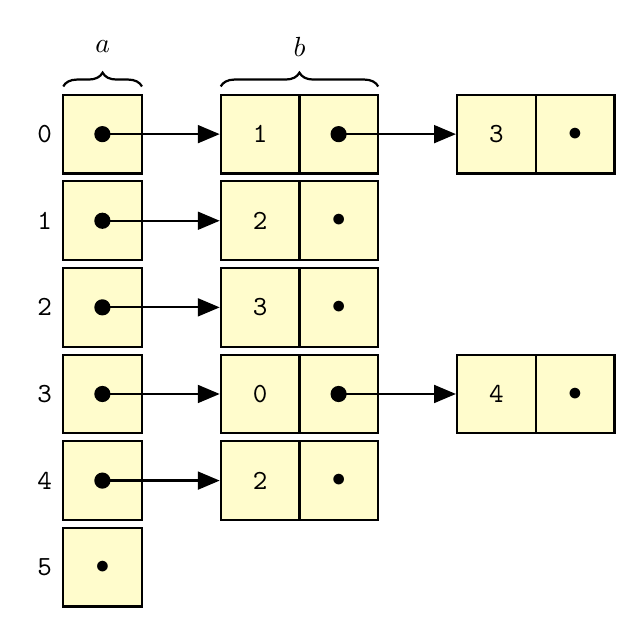
\begin{tikzpicture}[scale=1.00,transform shape]
\node[cell,label={left:0}] at (0.0,5.5) (a0) {};
\node[cell,label={left:1}] at (0.0,4.4) (a1) {};
\node[cell,label={left:2}] at (0.0,3.3) (a2) {};
\node[cell,label={left:3}] at (0.0,2.2) (a3) {};
\node[cell,label={left:4}] at (0.0,1.1) (a4) {};
\node[cell,label={left:5}] at (0.0,0.0) (a5) { $\bullet$};

\node[cell] at (2.0,5.5) (a0b1) {1};
\node[cell] at (2.0,4.4) (a1b1) {2};
\node[cell] at (2.0,3.3) (a2b1) {3};
\node[cell] at (2.0,2.2) (a3b1) {0};
\node[cell] at (2.0,1.1) (a4b1) {2};

\node[cell] at (3.0,5.5) (a0c1) {};
\node[cell] at (3.0,4.4) (a1c1) {$\bullet$};
\node[cell] at (3.0,3.3) (a2c1) {$\bullet$};
\node[cell] at (3.0,2.2) (a3c1) {};
\node[cell] at (3.0,1.1) (a4c1) {$\bullet$};

\node[cell] at (5.0,5.5) (a0d1) {3};
\node[cell] at (5.0,2.2) (a3d1) {4};

\node[cell] at (6.0,5.5) (a0e1) {$\bullet$};
\node[cell] at (6.0,2.2) (a3e1) {$\bullet$};



\draw[pointer] (a0b1) edge node {} (a0.center);
\draw[pointer] (a1b1) edge node {} (a1.center);
\draw[pointer] (a2b1) edge node {} (a2.center);
\draw[pointer] (a3b1) edge node {} (a3.center);
\draw[pointer] (a4b1) edge node {} (a4.center);

\draw[pointer] (a0d1) edge node {} (a0c1.center);
\draw[pointer] (a3d1) edge node {} (a3c1.center);

\draw [thick,decorate,decoration={brace,amplitude=5pt,raise=4ex}]
  (1.5,5.5) -- (3.5,5.5) node[midway,yshift=3em]{$b$};

\draw [thick,decorate,decoration={brace,amplitude=5pt,raise=4ex}]
  (-0.5,5.5) -- (0.5,5.5) node[midway,yshift=3em]{$a$};

% \node[rectangle, draw=none] at (0.0, 0.0) (a) {};
% \node[rectangle, thick, draw=black,minimum width = 1.0cm, minimum height =1.0cm,fill=red!20] at (3.2,0.0) (b) {$f$};
% \node[rectangle, thick, draw=black,minimum width = 1.0cm, minimum height =1.0cm,fill=red!20] at (6.8,0.0) (c) {$A_2$};
% \node[rectangle, draw=none] at (10.5, 0.0) (d) {};
% %
% \draw[thick,draw=black,->] (a) edge[above] node {$x \in I_1$} (b);
% \draw[thick,draw=black,->] (b) edge[above] node {$f(x) \in I_2$} (c);
% \draw[thick,draw=black,->] (c) edge[above] node {$s \in \{0,1\}$} (d);
\end{tikzpicture}




\end{document}